\usepackage{suthesis-2e}

\section{Conventional Particle Accelerators}

\section{Dielectric Laser Acceleration}

Dielectric laser accelerators (DLAs) are periodic dielectric structures that, when illuminated by laser light, create a near-field that may accelerate electrically charged particles such as electrons [england2014dielectric].
A principal figure of merit for these DLA structures is the acceleration gradient, which signifies the amount of energy gain per unit length achieved by a particle that is phased correctly with the driving field. 
DLAs may sustain acceleration gradients on the order of ${\sim}\textrm{GV}\,\textrm{m}^{-1}$ when operating using the high peak electric fields supplied by ultrafast (femtosecond) lasers.
These acceleration gradients are several orders of magnitude higher than conventional particle accelerators.
As a result, the development of DLA can lead to compact particle accelerators that enable new applications.

DLAs take advantage of the fact that dielectric materials have high damage thresholds at short pulse durations and infrared wavelengths \cite{england2014dielectric, mcneur2016elements, soong2012laser} when compared to metal surfaces at microwave frequencies.
This allows DLAs to sustain peak electromagnetic fields, and therefore acceleration gradients, that are 1 to 2 orders of magnitude higher than those found in conventional radio frequency (RF) accelerators.
Experimental demonstrations of these acceleration gradients have been made practical in recent years by the availability of robust nanofabrication techniques combined with modern solid state laser systems \cite{dawson2008analysis}.
By providing the potential for generating relativistic electron beams in relatively short length scales, DLA technology is projected to have numerous applications where tabletop accelerators may be useful, including medical imaging, radiation therapy, and X-ray generation \cite{plettner2008microstructure,england2014dielectric}.
To achieve high energy gain in a compact size, it is of principle interest to design structures that may produce the largest acceleration gradients possible without exceeding their respective damage thresholds.

Several recently demonstrated candidate DLA structures consist of a planar dielectric structure that is periodic along the particle axis with either an semi-open geometry or a narrow (micron to sub-micron) vacuum gap in which the particles travel \cite{plettner2006proposed, peralta2013demonstration, mcneur2016elements, leedle2015dielectric, chang2014silicon, breuer2014dielectric, breuer2014dielectric2, kozak2016dielectric}.
These structures are then side-illuminated by laser pulses. Fig.~\ref{fig:system} shows a schematic of the setup, with a laser pulse incident from the bottom.

\begin{figure}[htb!]
\centering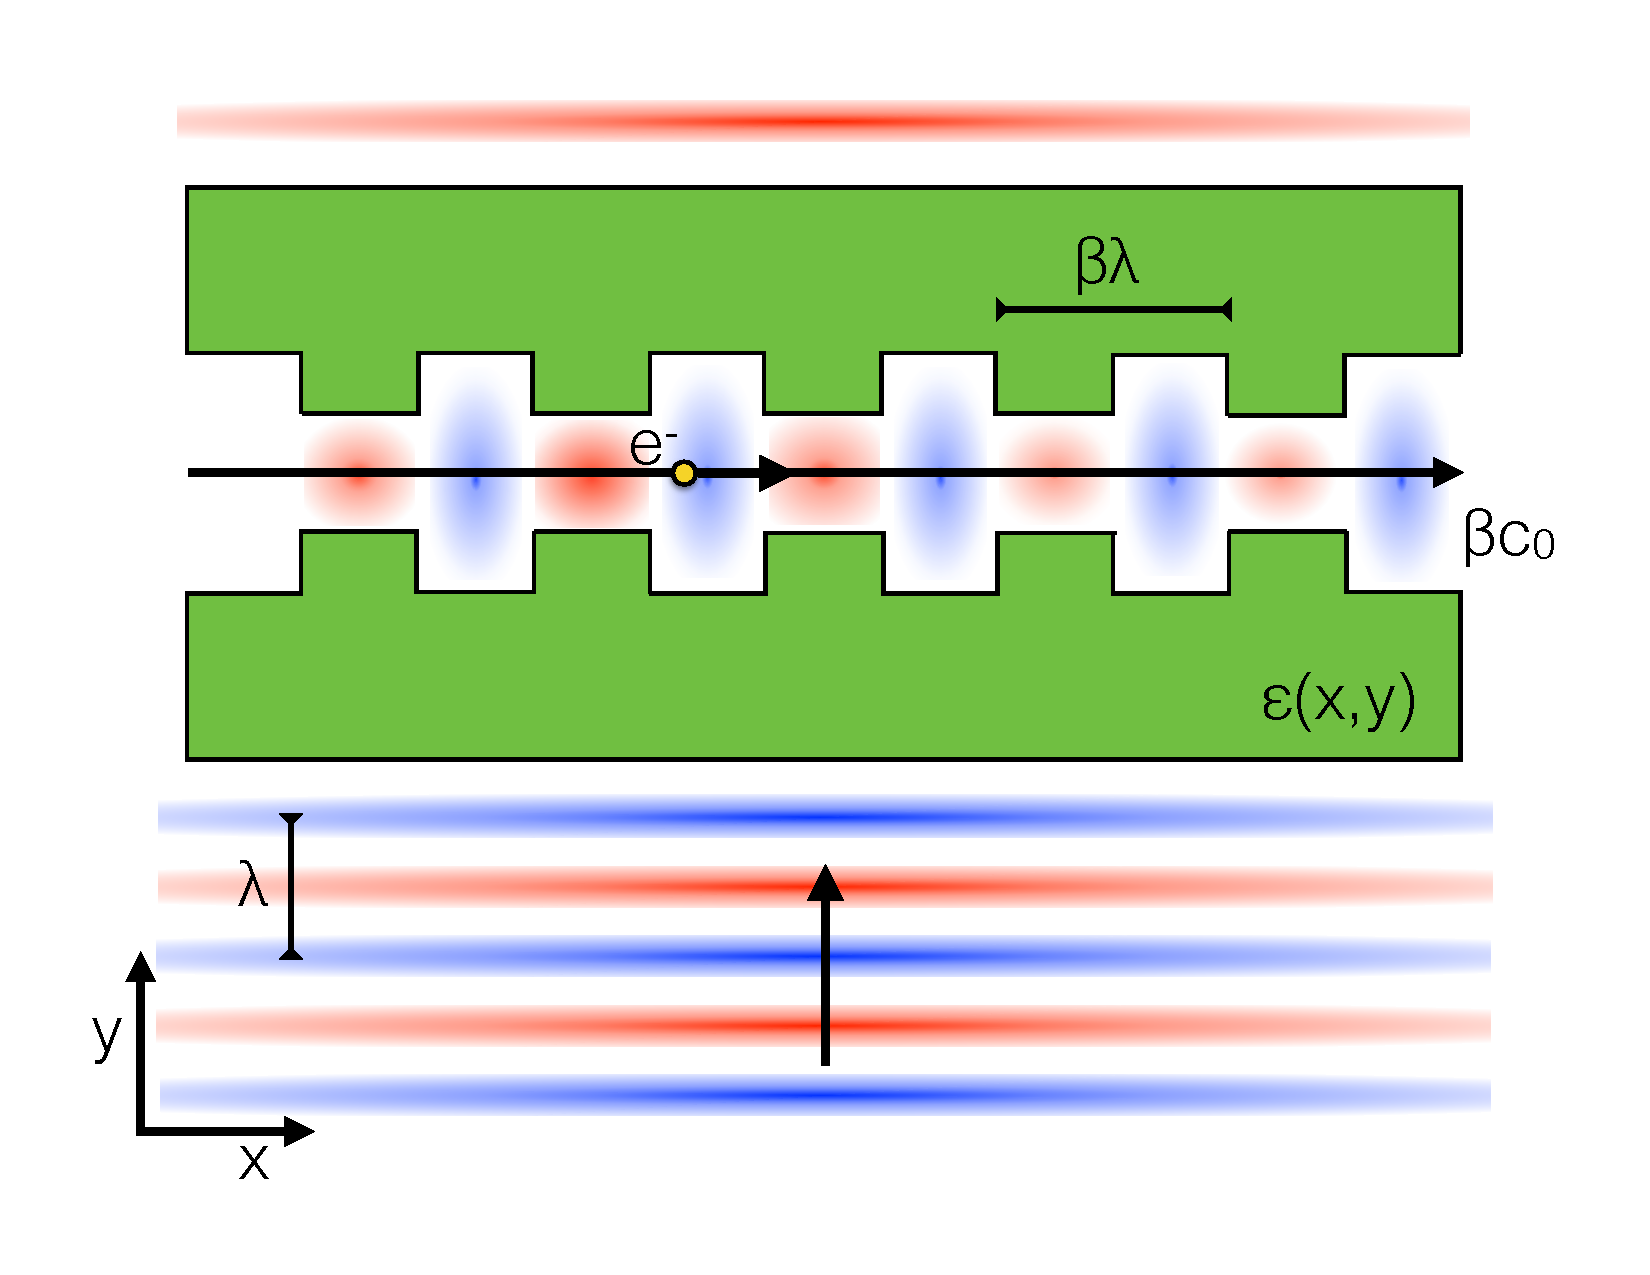
\includegraphics[width=\textwidth]{figures/DLA_definition.pdf}
\caption{Diagram outlining the system setup for side-coupled DLA with an arbitrary dielectric structure $\eps(x,y)$ (green).  A charged particle moves through the vacuum gap with speed $\beta c_0$.  The periodicity is set at $\beta \lambda$ where $\lambda$ is the central wavelength of the laser pulse.}
\label{fig:system}
\end{figure}

The laser field may also be treated with a pulse front tilt \cite{hebling1996derivation, akturk2004pulse} to enable group velocity matching over a distance greater than the laser's pulse length.
For acceleration to occur, the dielectric structure must be designed such that the particle feels an electric field that is largely parallel to its trajectory over many optical periods.
In the following calculations, the geometry of the dielectric structure is represented by a spatially varying dielectric constant $\eps(x,y)$.  We assume invariance in one coordinate ($\hat{z}$) in keeping with the planar symmetry of most current designs.
However the methodology we present can be extended to include a third dimension.
In addition, our work approximates the incident laser pulse as a monochromatic plane wave at the central frequency, which is a valid approximation as long as the pulse duration is large compared to the optical period.

\subsection{ACHIP Collaboration}
\subsection{Experimental Demonstrations}

\section{Design of Dielectric Laser Accelerator}

\subsection{Mathematical Definition}

In a general DLA system, we may define the acceleration gradient `$G$' over a time period `$T$' mathematically as follows:

\begin{equation}
G = \frac{1}{T}\int_0^{T}{ E_{||}(\vr(t),t)\ dt}
\label{eq:Gintro}
\ ,
\end{equation} 
where $\vr(t)$ is the position of the electron and $E_{||}$ signifies the (real) electric field component parallel to the electron trajectory at a given time.

Since the structure is invariant in the $\hat{z}$ direction, we work in two dimensions, examining only the $H_z$, $E_x$ and $E_y$ field components.
For an approximately monochromatic input laser source with angular frequency $\omega$, the electric fields are, in general, of the form


\begin{equation}
\bfx(\vr,t) = \real{\bfx(\vr)e^{i\omega t}},
\end{equation}
where now $\bfx$ is complex.

Let us assume the particle we wish to accelerate is moving on the line $y=0$ with velocity $\vec{v} = \beta c_0 \hat{x}$, where $c_0$ is the speed of light in vacuum and $\beta \leq 1$.
The $x$ position of the particle as a function of time is given by $x(t) = x_0 + \beta c_0 t$, where $x_0$ represents an arbitrary choice of initial starting position.
For normal incidence of the laser (laser propagating in the $+\hat{y}$ direction), phase velocity matching between the particle and the electromagnetic fields is established by introducing a spatial periodicity in our structure of period $\beta \lambda$ along $\hat{x}$ , where $\lambda$ is the laser wavelength.
In the limit of an infinitely long structure (or equivalently, $T \to \infty $) we may rewrite our expression for the gradient in Eq. (\ref{eq:Gintro}) as an integral over one spatial period, given by

\begin{equation}
G = \frac{1}{\beta\lambda}\real{ e^{-i\phi_0}\int_0^{\beta\lambda}{dx \ }E_x(x,0)e^{i\frac{2\pi}{\beta\lambda}x}}.
\end{equation}
%
Here the quantity $\phi_0 = \frac{2\pi x_0}{\beta\lambda}$ is representative of the phase of the particle as it enters the spatial period.
In further calculations, we set $\phi_0 = 0$, only examining the acceleration gradients experienced by particles entering the accelerator with this specific phase.
Since we have arbitrarily control over our input laser phase, this does not impose any constraint on the acceleration gradient attainable.

To simplify the following derivations, we define the following inner product operation involving the integral over two vector quantities $\va$ and $\vb$ over a single period volume $V'$

\begin{equation}
\bracket{\va}{\vb} = \int_{V'} dv \  \left(\va \cdot \vb \right) = \int_0^{\beta\lambda}dx\int_{-\infty}^\infty dy \left(\va\cdot\vb\right).
\end{equation} 
With this definition, we then have the gradient

\begin{equation}
G = \real{\bracket{\vE}{\veta}},
\label{eq:G}
\end{equation}
where

\begin{equation}
\veta(x,y) = \frac{1}{\beta\lambda}e^{i\frac{2\pi}{\beta\lambda}x}\delta(y)\hat{x}.
\end{equation}

Our goal in designing the accelerator is thus to create a permittivity distribution that maximizes $G$ subject to a few constraints.
First, we require that a small gap exist for the electron to travel through the structure.
Secondly, we assume that the structure has a finite extent along the direction of the incoming laser beam.
We also consider realizing this device through the patterning of a material with permittivity $\eps_\textrm{max}$.  
Therefore, the final device should have permittivity of either 1 or $\eps_\textrm{max}$ at all points.

\subsection{Brute Force Method}

To solve such a problem, we may first define a design region in which we allow the permittivity to vary.
For the purposes of this example, we consider two slabs surrounding the central accelerator gap, as diagrammed in Fig. [To Do].

We now may consider discretizing our entire spatial domain into a rectangular grid, which will be necessary for numerical simulation.
This also allows us to define our design parameters as the permittivity of each grid cell within the design region.  Thus, the goal is to find the permittivity of each pixel that will maximize the acceleration gradient, subject to each grid cell having a permittivity value of either 1 or $\eps_\textrm{max}$.

To accomplish this, the simplest approach would involve doing a direct search over the full design space.  For example, one could label each cell within the design region with an identifier `0' or `1' corresponding to `vaccuum' and `material', respectively.  Then, one may generate all possible structures and check their respective acceleration gradients.

However, as one can imagine, this method would be far too computationally expensive to perform in practice.
For example, even considering a very small design region consisting of 10 $\times$ 10 = 100 grid cells would result in $2^{100} \approx 10^{30}$ devices to simulate.
While one may consider smart ways of searching through this device space without checking each structure, using global optimization approaches such as genetic algorithms [memetic] or particle swarm optimization [particle swarm], this problem is still quite computationally expensive and is exponentially worse as the number of design parameters are increased.

\subsection{Gradient-based Optimization}

A smarter approach involves $\textit{gradient-based optimization}$, in which we search the design space according to the local gradient of the figure of merit with respect to each of the parameters.
For example, we may start with an initially random device, compute how the performance will change with respect to a change in the permittivity of each cell in the design region, and make a small update.
This process may be repeated until convergence on a locally optimal solution.
If the design space contains several local optima, then this whole process may be repeated several times with different initial conditions.

In fact, this method is the standard approach to training of neural networks, which may also be framed as an optimization problem over thousands to millions of parameters.
We will revisit this connection in a later chapter.
While the performance of gradient-based optimization is hard to directly compare to that of global optimization approaches, as the number of design parameters increases, gradient-based optimization are typically preferred as they require far fewer steps in most problems [cite].
% expand on this?

For gradient-based optimization to be useful, one would like an efficient means to compute the gradient of the figure of merit with respect to the design parameters.
For neural networks, the gradient is computed analytically and then evaluated using the \textit{backpropagation} algorithm [cite backprop].
For photonic devices, one may perform a similar technique using the \texit{adjoint method}, which allows one to analytically compute the gradient directly from Maxwell's Equations and evaluate the result with only one additional electromagnetic simulation.
This remarkable efficiency is largely responsible for the success of inverse design in photonics.

\section{Adjoint Method}

The adjoint method is typically introduced for linear optical systems, although, as we will show in a later chapter, it may be extended to nonlinear systems without much additional effort.
In the frequency domain, Maxwell's equations may be written as

\begin{equation}
\dcurl \vE (\vr)\ -\ k_0^2\ \eps_r(\vr)\ \vE(\vr) \equiv A\vE(\vr) = -i\mu_0\omega\vJ(\vr),
\label{eq:FDFD_analytical}
\end{equation}
%
Here, $\vE(\vr)$ and $\vJ(\vr)$ are the electric field and electric current distributions, respectively. $k_0 = \omega/c_0$, $\eps_r$ is the relative permittivity and a non-magnetic material is assumed ($\mu = \mu_0$)

More abstractly, we may write Eq. (\ref{eq:FDFD_analytical}) as
%
\begin{equation}
A \bfx = \bfb,
\label{eq:FDFD_simple}
\end{equation}
%
where $A$ is a sparse, complex symmetric matrix that encodes Maxwell's equations on the device.  
$\bfx$ is a vector containing the electromagnetic fields at each position in the domain, which are the solution to Eq. (\ref{eq:FDFD_simple}) given the vector $\bfb$ describing the electric current source distribution in the domain.

Our device is described by a set of design variables $\bm{\phi}$, which influence the system matrix, $A = A(\bfphi)$.
Differentiating \eq{eq:FDFD_analytical} with respect to $\bfphi$, and assuming that the current source, $\bfb$, does not depend on $\bfphi$, we may recover the change in the solution with respect to the parameters as
%
\begin{equation}
\dfrac{\bfx}{\bfphi} = -\invA \pfrac{A}{\bfphi} \invA \bfb = -\invA \pfrac{A}{\bfphi}\bfx
\label{eq:dEdgamma}.
\end{equation}
%
Now, we consider differentiating an objective function $J = J(\bfx)$ that depends explicitly on the field solution.
By the chain rule, this gives

\begin{equation}
\dfrac{J}{\bfphi} =  - \real{ \pfrac{J}{\bfx} \dfrac{\bfx}{\bfphi} } = - \real{ \pfrac{J}{\bfx} A^{-1} \pfrac{A}{\bfphi} \bfx }
\label{eq:dGdgamma_2}.
\end{equation}

To evaluate \eq{eq:dGdgamma_2}, we define a second simulation with source term $-\pfrac{J}{\bfx}^T$,

\begin{equation}
A^T\bfx_\aj = A\bfx_\aj = -\pfrac{J}{\bfx}^T,
\label{eq:adjoint_source}
\end{equation}
then the field solution, $\bfx_\aj = -A^{-1}\pfrac{J}{\bfx}^T$, can be easily identified in \eq{eq:dGdgamma_2}, which gives the expression

\begin{equation}
\dfrac{G}{\bfphi} = \real{ \bfx_\aj^T \pfrac{A}{\bfphi} \bfx }.
\label{eq:final_form_DGdgamma}
\end{equation}

The only quantity in this expression that depends on the parameter $\bfphi$ is $\pfrac{A}{\bfphi}$.  As we will soon discuss, this quantity will generally be trivial to compute.
On the other hand, the full field calculations of $\bfx$ and $\bfx_\aj$ are computationally expensive, but may be computed once and used for an arbitrarily large set of parameters $\bfphi_i$.
This gives the adjoint method significant scaling advantage with respect to traditional direct sensitivity methods, such as finite difference, which require a separate full-field calculation for each parameter being investigated.

\subsection{Application to Accelerator}



\section{Inverse design of Dielectric Laser Accelerator}{}

\subsection{Optimization Routine}

\subsection{Results and Comparison to Existing Structures}

\subsection{Interpretation of Adjoint Fields as Radiation}
